\subsubsection{Introduction}

For Part a, the given ``VGG-lite'' CNN structure (Figure
\ref{fig:images-vgglite}) must be implemented. This model will act as a base for
each of the subsequent parts in section 1. The given structure has 9 layers,
takes the input images, which are of size 224x224, and outputs a classification
based on one of the six classes.

\begin{figure}[H]
	\centering
	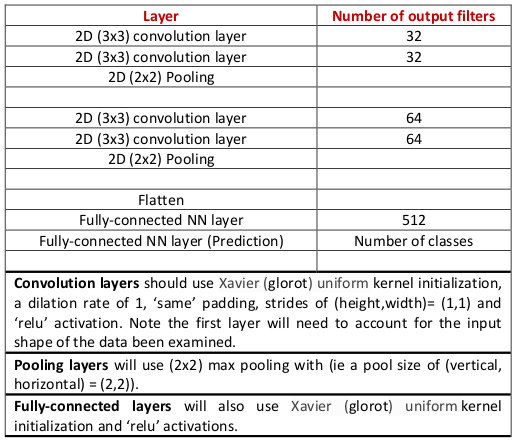
\includegraphics[width=0.8\textwidth]{images/vgglite}
	\caption{Given VGG-lite Structure}
	\label{fig:images-vgglite}
\end{figure}

\subsubsection{Design}

The first steps in implementing
this system is loading the data into Google Colab. This functionality is
available through the ``google.colab'' ``drive'' library. The required directory
must be mounted to the session, and the zipped data must be extracted. The code
implementation in Figure \ref{fig:unzip} shows this functionality.

\begin{figure}[H]
	\centering
	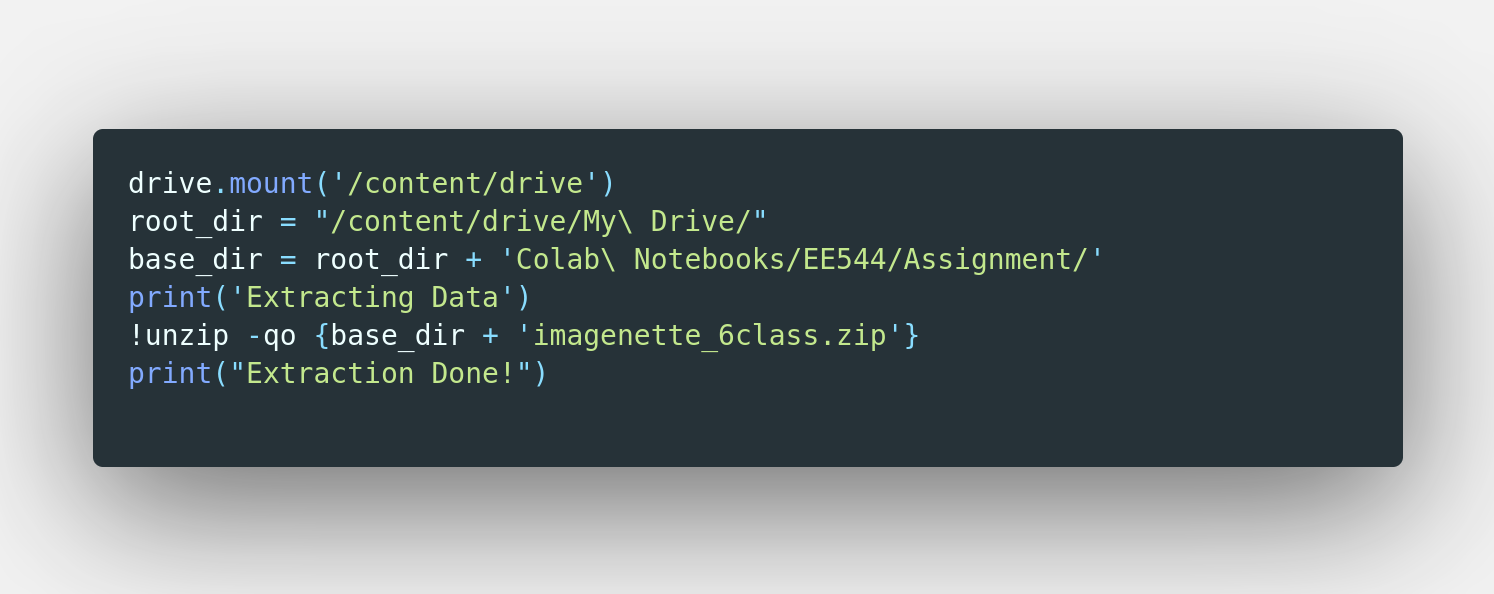
\includegraphics[width=0.8\textwidth]{images/Code/loadData}
	\caption{Extract Data from ZIP File}
	\label{fig:unzip}
\end{figure}

To load data from a directory, Tensorflow Keras provides the
``flow\_from\_directory'' method. This method takes a directory, image size, and
class mode. For the given dataset, the directories are ``train'',
``validation'', and ``test''. The target size for each of the images is 224x224,
and the class mode is ``categorical'', as there are multiple classes of output.
For the test data, the class mode must be set to ``None'', and the data must not
be shuffled, as specified by the arguement ``shuffle=False''.

\begin{figure}[H]
	\centering
	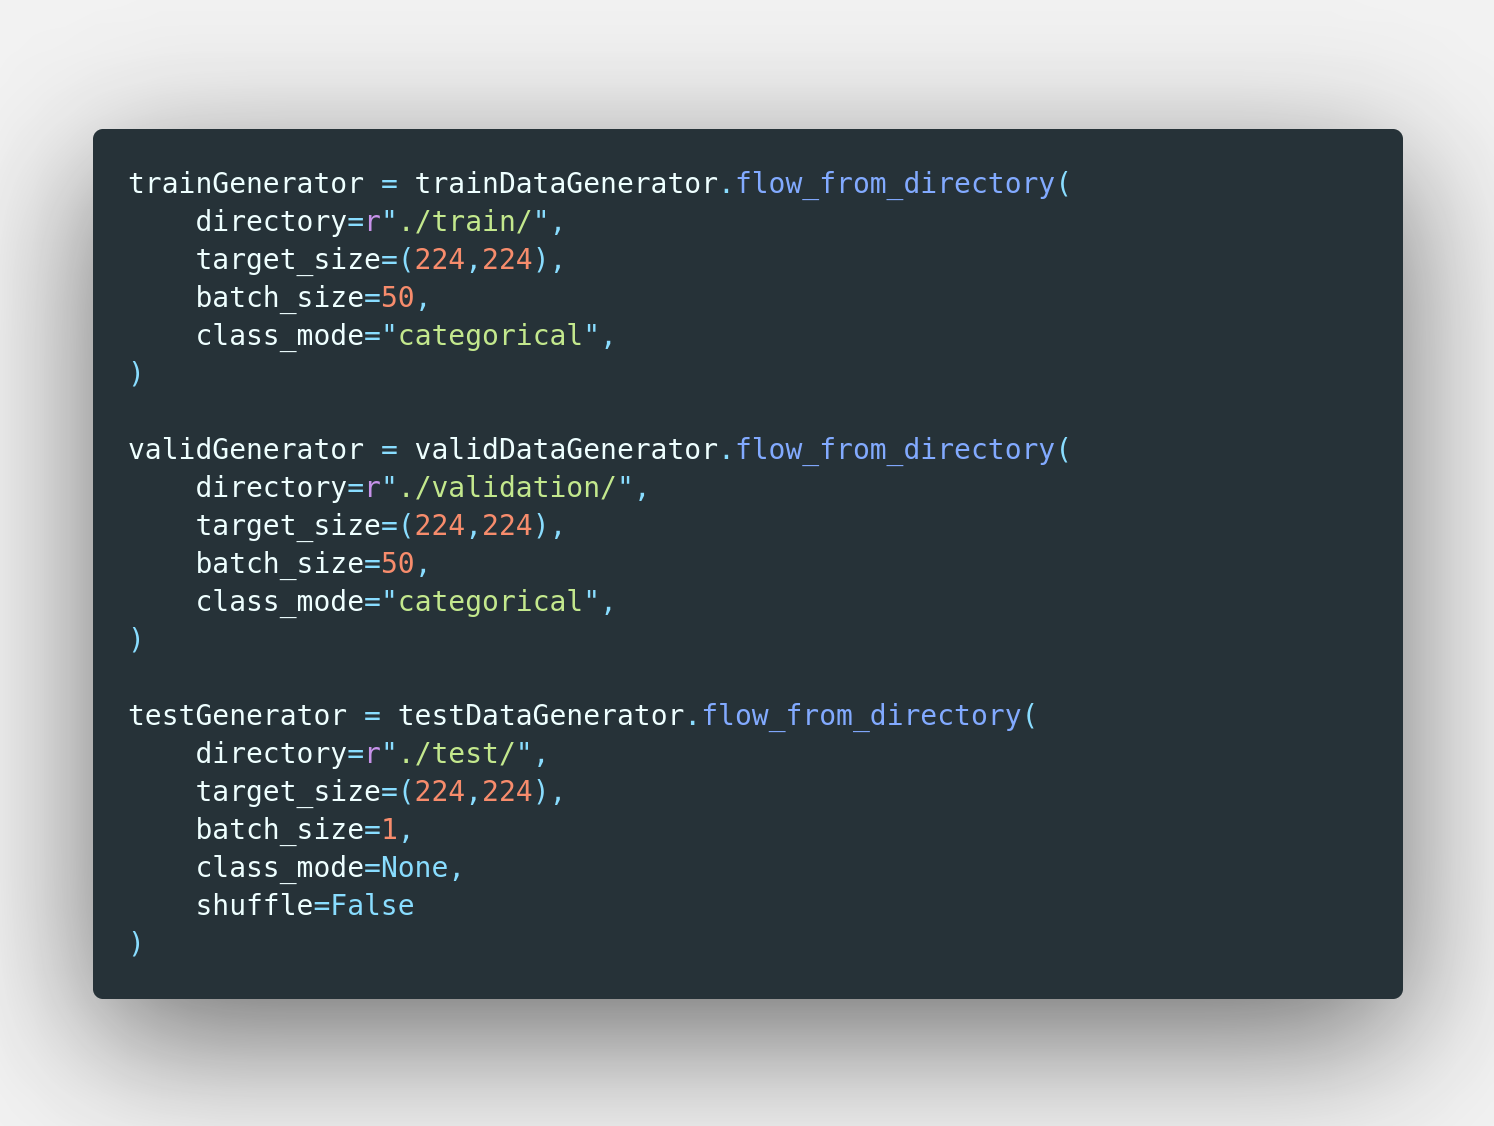
\includegraphics[width=0.8\textwidth]{images/Code/loadDataFromDir}
	\caption{Load in Data from Directory}
	\label{fig:flow}
\end{figure}

To construct the neural network, the ``model.add'' method is called to add
layers. Layers are added as previously specified. The 2D convolutional layers
have 32 output filters, a 3x3 kernel, a stride of 1, padding ``same'', ``relu''
activation, and ``glorot\_uniform'' kernel initialization. There is a difference
with the input layer, which must specify the input shape in the form (rows,
columns, channels). In this case, the input shape is 244x244x3. These layers are
added as Keras ``Conv2D'' layers.

Following the 2D convolutional layer is a 2D pooling layer. This is implemented
with the ``MaxPooling2D'' function, which takes a pool size as an input. In this
case, the specified pool size is 2x2. There are two additional 2D convolutional
layers, with 64 output filters, followed by another 2D pooling layer.

A Flatten layer is added before the fully connected layers of the model. The
Keras ``Flatten'' function takes no input arguements.

Each of the final Dense layers use the ``glorot\_uniform'' kernel initializer.
The first Dense layer has 512 output units and ``relu'' activation. The final
layer must have 6 output units, as there are 6 total classification classes. It
uses ``softmax'' activation. This must also be used, as ReLU has very poor
performance as an output layer.

The finalized neural network is shown in Figure \ref{fig:q1Model}.

\begin{figure}[H]
	\centering
	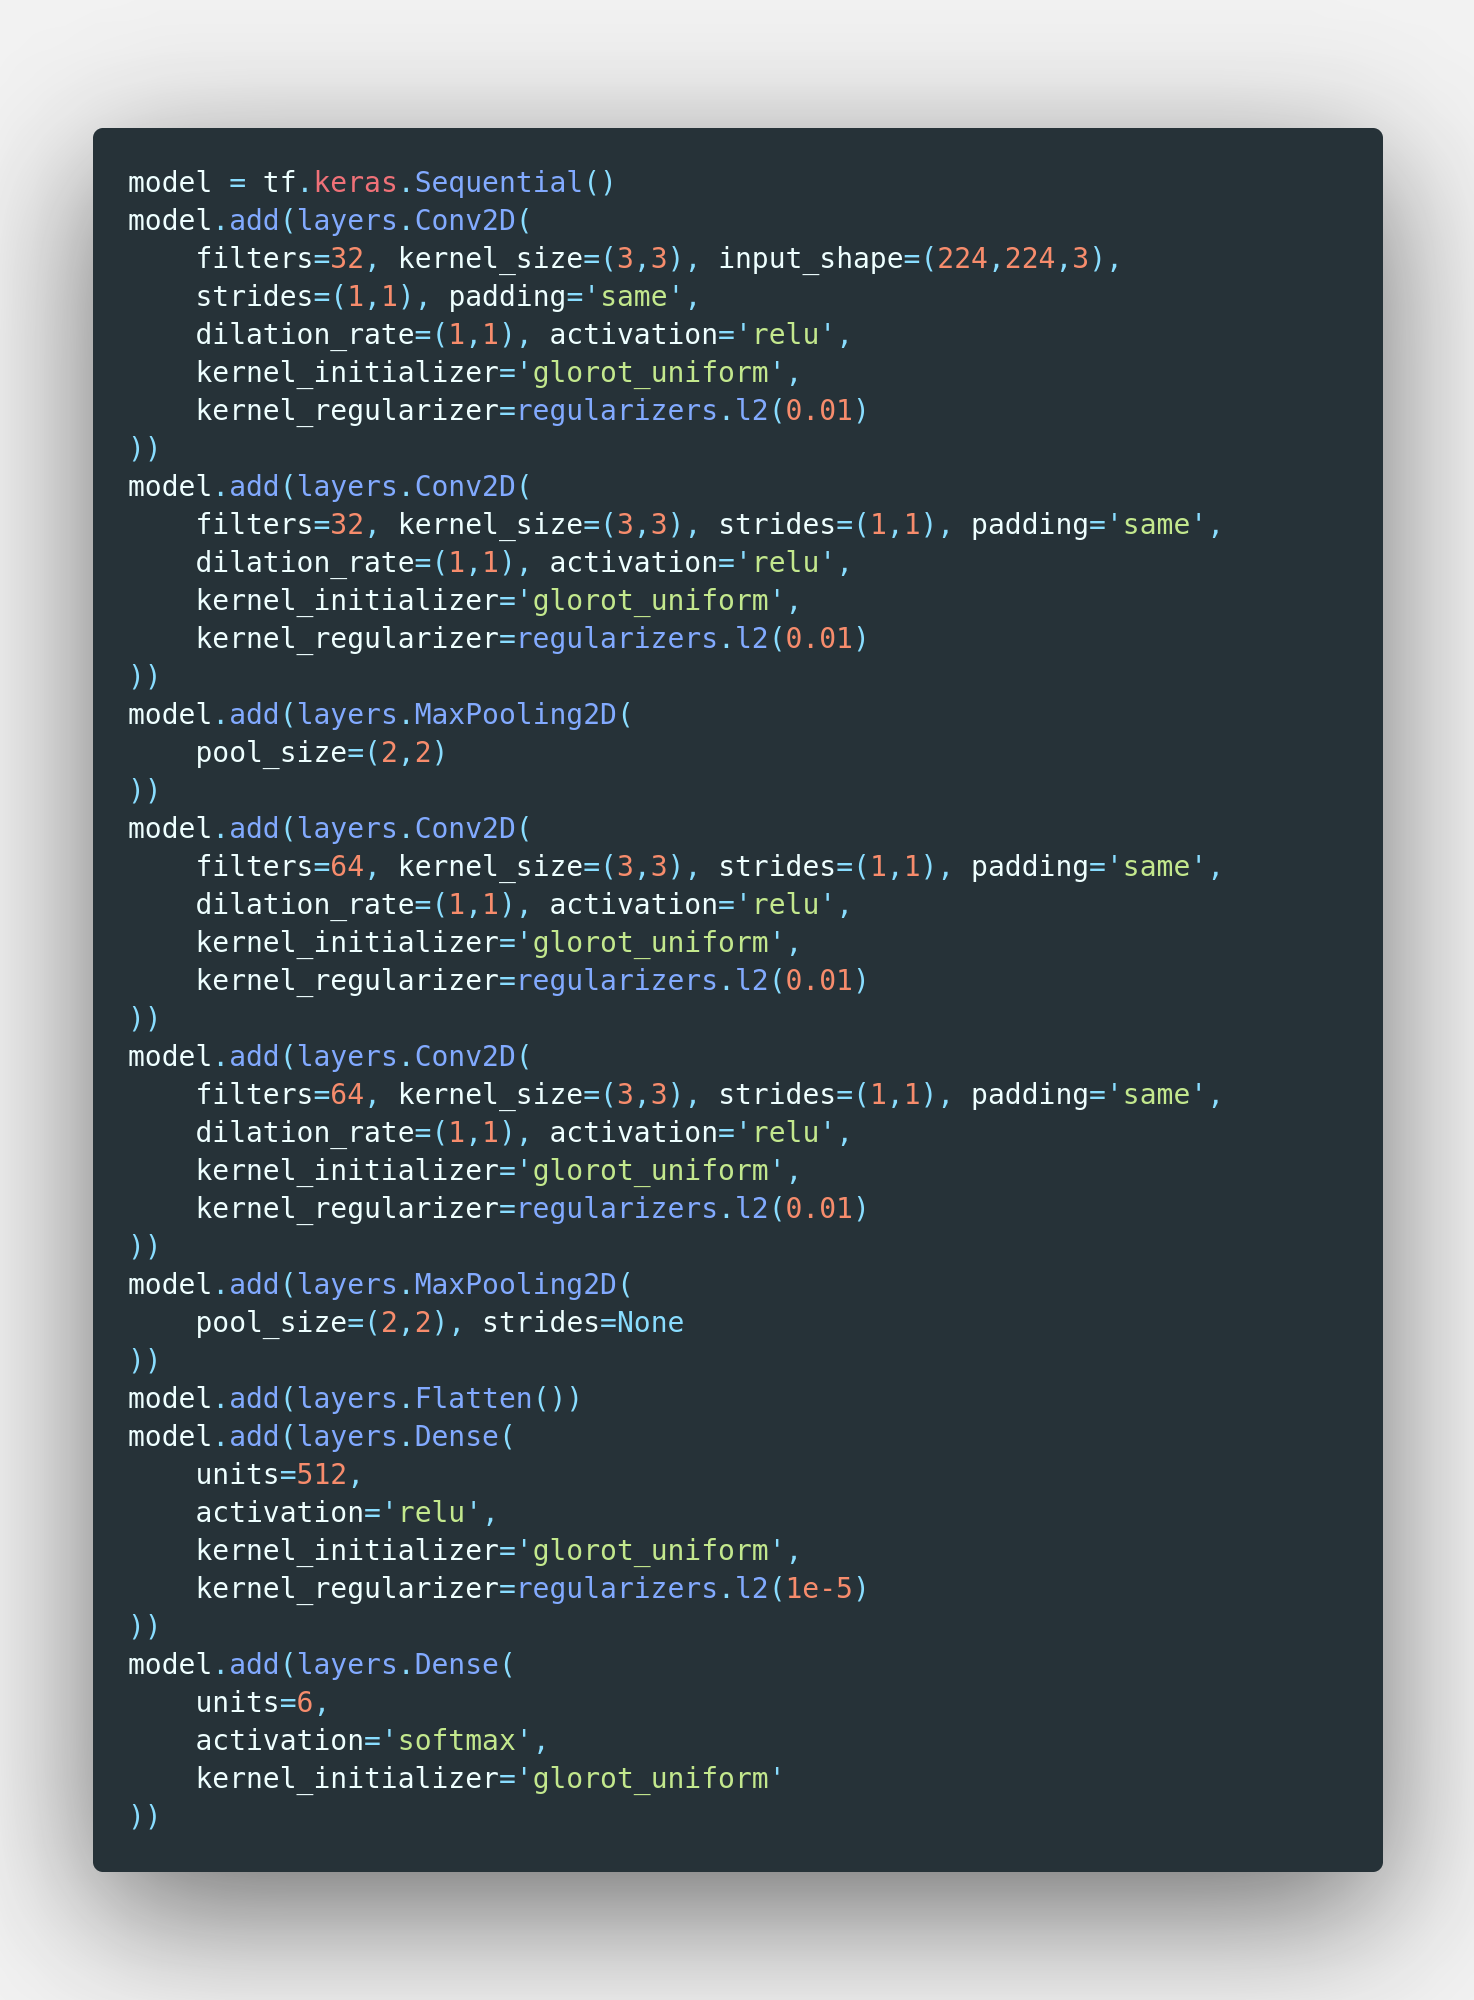
\includegraphics[width=0.8\textwidth]{images/Code/model}
	\caption{Question 1 Base Model}
	\label{fig:q1Model}
\end{figure}

\subsubsection{Testing}

There are a number of hyperparameters which may be tuned for this model. Each
``Conv2D'' and ``Dense'' layer have activity regularizers, kernel regularizers,
and bias regularizers which can be modified in order to tune the performance of
the neural network.

Manual tuning was performed for these hyperparameters for various input values.
This was done due to a lack of understanding of the ``kerastuner'' tool, which
allows for automated hyperparameter selection.In order to shorten the amount of
time taken for testing, early stopping was implemented, which stops training
when there has been no change in the validation loss in a set number of epochs.
5 epochs was chosen as the limit for this.

Kernel regularizers were the hyperparameters which were utilised for the purpose
of tuning. A number of values for the hyperparameters were tested, with the
validation accuracy used as the metric by which they were compared.

First, the kernel regularizer for the final ``relu'' activated Dense layer was
tested, this is labelled as ``Regularizer Value'' within the following table.
The regularizer chosen for the purpose of this section was the ``l2'' ``weight
decay'' regularizer.
The kernel regularizer for each other layers was set to a value of 0.01,
while the Dense layer regularizer was modified in order to obtain the highest
possible accuracy.

\begin{table}[H]
	\centering
	\caption{Kernel Regularizer Hyperparameter Tuning (Final ``ReLU'' Dense
	Layer)}
	\label{tab:krhyp}
	\begin{tabular}{|c|c|}
	\hline
	Regularizer Value & Validation Accuracy \\
	\hline
	0.00005 & 69.17 \\
	0.00001 & 71.83 \\
	0.0005  & 76 \\
	0.00025 & 77 \\
	0.0001  & 70 \\
	\hline
	\end{tabular}
\end{table}

As given by the output listed above, the regularizer value of 0.00025 gave the
highest validation accuracy, and as such was used moving forward. The kernel
regularizer value of the other layers were then tested, as shown in the table
below.

\begin{table}[H]
	\centering
	\caption{Kernel Regularizer Hyperparameter Tuning (Other Layers)}
	\label{tab:krhypo}
	\begin{tabular}{|c|c|}
	\hline
	Regularizer Value & Validation Accuracy \\
	\hline
	0.001 & 74 \\
	0.005 & 75 \\
	0.0005 & 73 \\
	``None'' & 77 \\
	\hline
	\end{tabular}
\end{table}

As the optimal value is shown to be ``None'', i.e. no regularizer is used, this
is the option used for the model. While these options are the optimum arrived at
using manual hyperparameter tuning, there may be more optimal choices.

Another hyperparameter which must be chosen is the learning rate of the chosen
optimizer. For this section, the ``Adam'' optimizer was chosen, as the
hyperparameter tuning is relatively easy, especially when being done manually.

\begin{table}[H]
	\centering
	\caption{Learning Rate Hyperparameter Tuning}
	\label{tab:lrhyp}
	\begin{tabular}{|c|c|}
	\hline
	Learning Rate & Validation Accuracy \\
	\hline
	0.01 & 16.67 \\
	0.001 & 71.33 \\
	0.0001 & 74.83 \\
	0.00001 & 74.33 \\
	\hline
	\end{tabular}
\end{table}

The learning rate value of 0.0001 was selected, as it gave the highest value for
validation accuracy. With this value, the final model could be tested.

For the purposes of training, the model was set to train for 30 epochs, however,
the value for early stopping patience was increased from 5 to 7, in order to
prevent overfitting without stopping too early to train correctly.

\subsubsection{Results}

The correct output for the neural network structure was printed using the
``model.summary'' function in keras, as seen in Figure \ref{fig:q1paModSum}.
This shows the output shape of the final layer as 6, which is the number of
possible classifications, along with all of the specified outputs in all other
layers.

\begin{figure}[H]
	\centering
	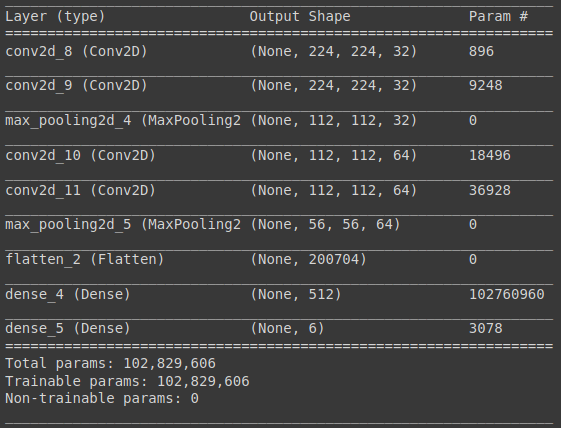
\includegraphics[width=0.8\textwidth]{images/q1/pa/q1pamodel}
	\caption{Model Summary}
	\label{fig:q1paModSum}
\end{figure}

It is clear from both Figures \ref{fig:q1paAcc} and \ref{fig:q1paLoss} that
overfitting does not occur within this model. The validation accuracy of the
model reaches approximately 80\%, however, the loss value reaches approximately
2.00. The final output, as shown in Figure \ref{fig:q1paRes} shows a final
validation accuracy of 79.50\%.

\begin{figure}[H]
	\centering
	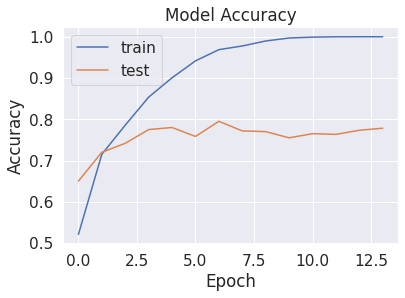
\includegraphics[width=0.8\textwidth]{images/q1/pa/accuracy}
	\caption{Validation and Training Acccuracy}
	\label{fig:q1paAcc}
\end{figure}

While the validation accuracy is trending upwards, it is possible that better
tuning of the hyperparameters would give a higher validation accuracy.

\begin{figure}[H]
	\centering
	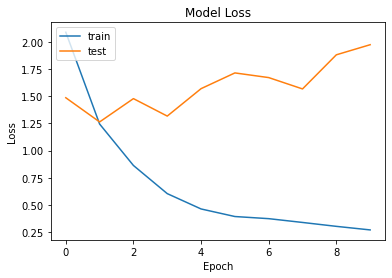
\includegraphics[width=0.8\textwidth]{images/q1/pa/loss}
	\caption{Validation and Training Loss}
	\label{fig:q1paLoss}
\end{figure}

The validation loss continues to rise. It is again possible that this could be
attributed to incorrect hyperparameter tuning.

The final output shows an average precision and recall of 81\%, with the highest
values attributed to the ``Parachute'' class, and the lowest values attributed
to the ``English Springer'' class.

\begin{figure}[H]
	\centering
	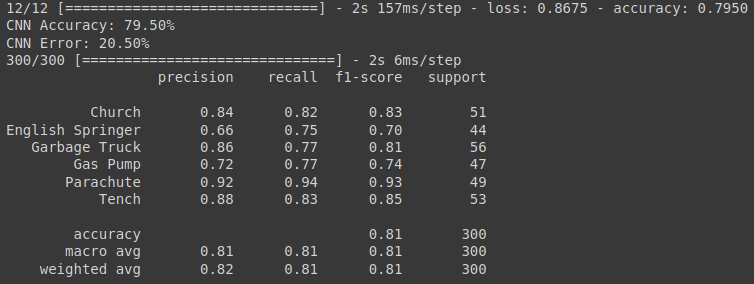
\includegraphics[width=0.8\textwidth]{images/q1/pa/results}
	\caption{Model Testing Results}
	\label{fig:q1paRes}
\end{figure}

The final confustion matrix, as shown in Figure \ref{fig:q1paMatrix}, shows the
number of correctly identified samples in testing, and as previously noted, the
class with the highest precision and recall is ``Parachute'' labelled as ``4''
within the matrix.

\begin{figure}[H]
	\centering
	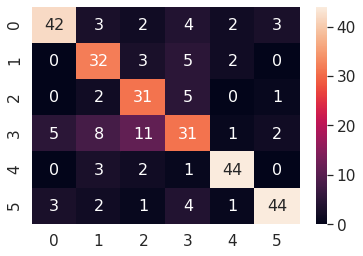
\includegraphics[width=0.8\textwidth]{images/q1/pa/matrix}
	\caption{Confusion Matrix}
	\label{fig:q1paMatrix}
\end{figure}

Using early stopping, the model ran for a total of 14 epochs. The training time
for the model was 436.109 seconds. Given that 1 hour of training on an Nvidia
GPU produces approximately 0.25lbs of CO2 equivalent emissions, this training
has an emission output of 0.03lbs CO2 equivalent emissions.
